\documentclass[12pt,a4paper]{article}
\usepackage[table]{xcolor}
\usepackage{float}
\usepackage[spanish]{babel}
\usepackage{amsmath}
\usepackage{amssymb}
\usepackage{graphicx}
\usepackage{amsfonts}
\usepackage[utf8]{inputenx}
%\usepackage{algorithm2e}
\usepackage{listings}
\usepackage{pdfpages}
\usepackage{tabularx}
\usepackage{color}
\usepackage{anysize}
\usepackage{fancyhdr}
%\usepackage{caption}
\usepackage[font=footnotesize]{caption}
\definecolor{deepblue}{RGB}{0,0,153}
\definecolor{deepred}{RGB}{153,0,0}
\definecolor{deepgreen}{RGB}{51,102,0}
\definecolor{deepyellow}{RGB}{204,204,0}
\marginsize{2cm}{2cm}{1cm}{1.5cm} % depende de anysize
%\renewcommand*{\thefootnote}{\Roman{footnote}}
\lstset{ %
			language=Python,
			basicstyle=\footnotesize,
			numbers=left,
			stepnumber=1,
			numbersep=4pt,
			tabsize=2,
			otherkeywords={self}, 
			keywordstyle=\color{deepred},
			stringstyle=\color{deepgreen},
			commentstyle=\color{deepblue},
}
\usepackage{hyperref}
\hypersetup{
    colorlinks=true,
    citecolor=black,
    filecolor=black,
    linkcolor=black,
    urlcolor=black,
    linktoc=all
}



%\title{Multímetros en Corriente Continua}
\title{TP Final}
\author{
        Grupo 1
}
\date{\today}
\pagestyle{fancy}
\lhead{Facultad de Ingenieria}
\rhead{Laboratorio - 66.02 - Curso 001 - TP Final}


\begin{document}
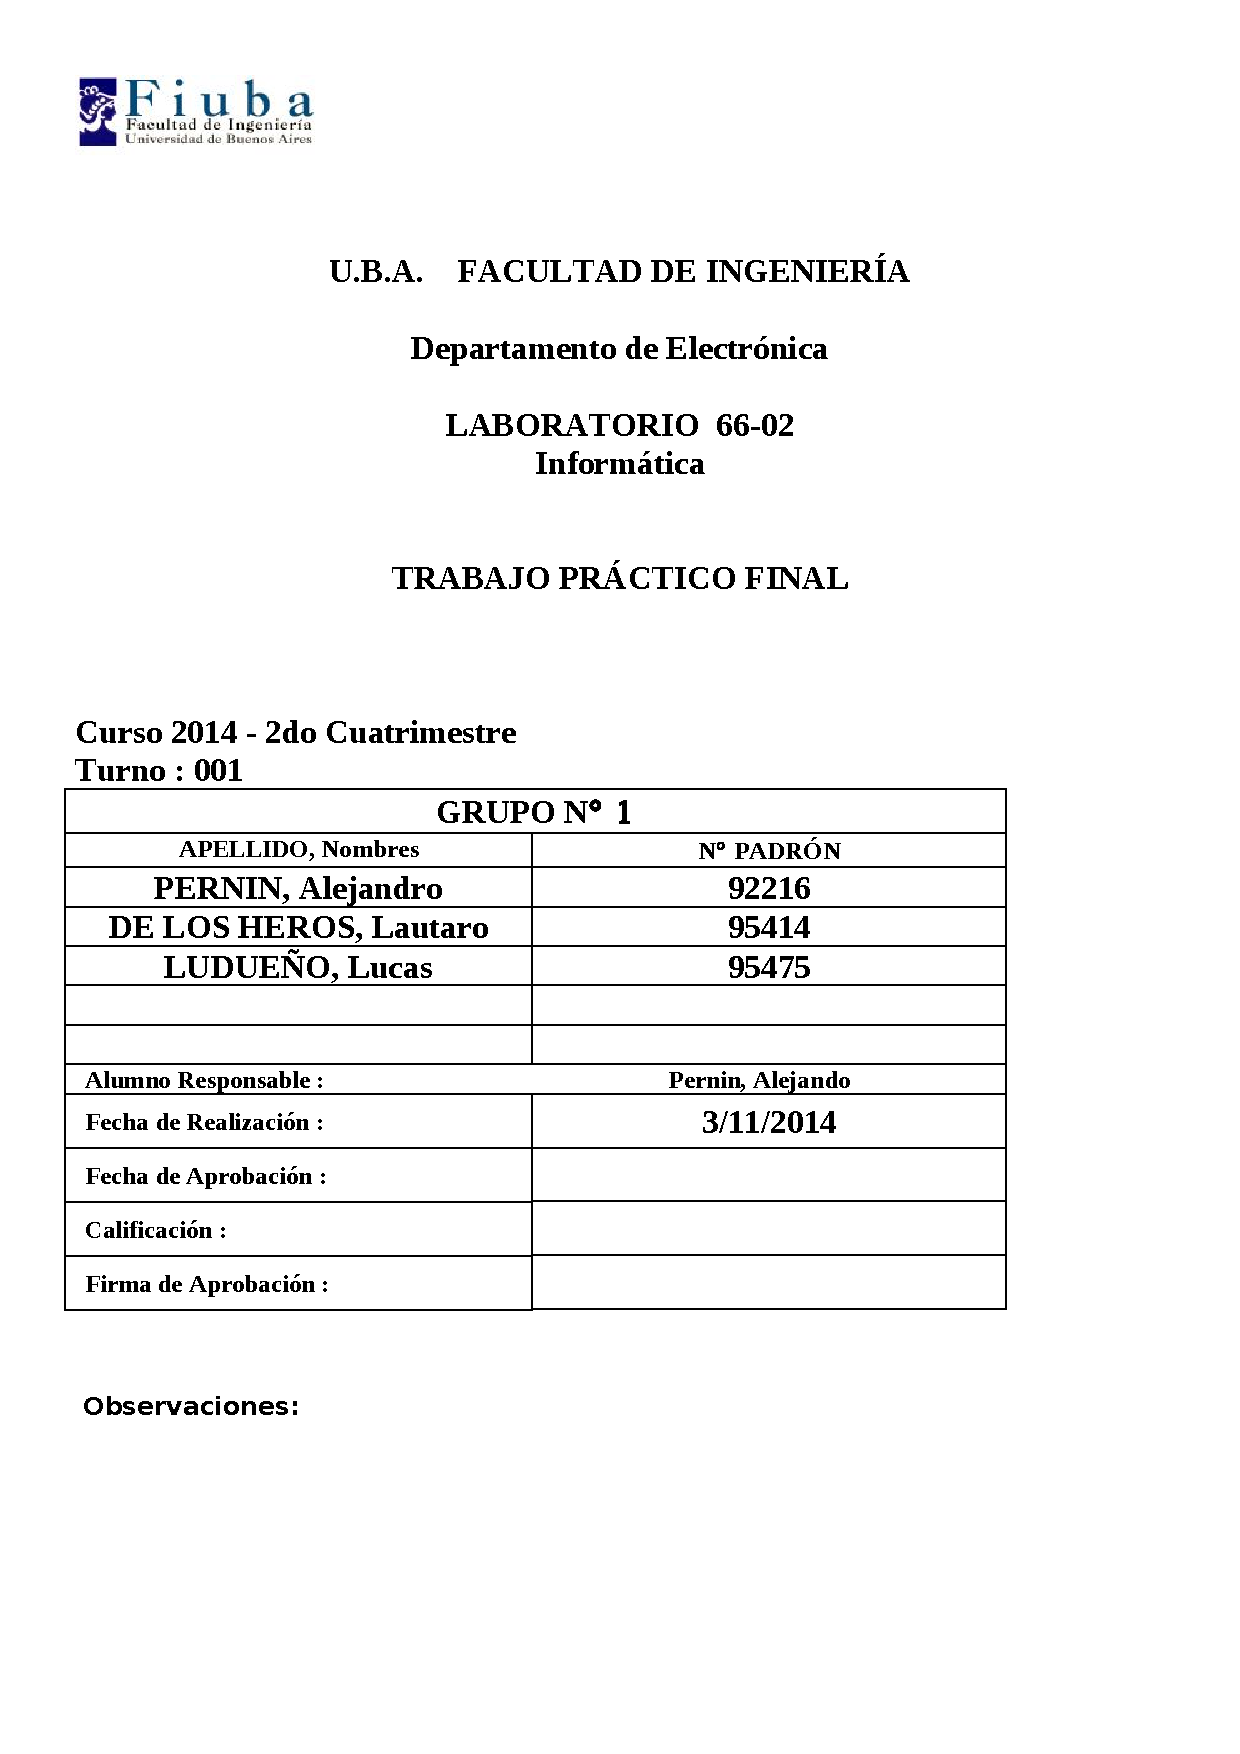
\includepdf{caratula.pdf}

\maketitle

\newpage
\tableofcontents

\newpage


\newpage 
\section{Introducción}
	El objetivo de este informe es exponer el trabajo práctico final, mostrando los desarrollos, mediciones efectuadas, funcionamiento y decisiones tomadas durante la confección del mismo. Éste fue realizado a lo largo del cuatrimestre en paralelo con las clases prácticas y los otros trabajos prácticos. Todos los archivo aquí utilizados, incluyendo este informe y su fuente estarán disponibles en \url{http://github.com/aleperno/labotpfinal}. Adicionalmente habrán disponibles algunos videos en YouTube con filmaciones de determinadas mediciones, por lo que es recomendable tener este informe en formato digital para fácil acceso a dichos links.

	\subsection{Opciones Disponibles}
		Habiendo diversas alternativas de proyectos de TPs para elegir, en un principio no estuvo del todo claro cuál elegir ya que todos tenian sus complicaciones y objetivos. Algunas de las alternativas disponibles eran la confección de una fuente, un sensor, etc.

	\subsection{Opción Elegida}
		Como proyecto base decidimos desarrollar un voltímetro vúmetro disponible en los cursos de CEKIT \footnote{Pdf del proyecto oringal \url{https://github.com/aleperno/labotpfinal/raw/master/cekit.pdf}}. Elegimos este proyecto ya que si bien se trata de un proyecto relativamente sencillo, tiene aplicaciones reales tanto industriales como hogareñas.

		Además aprovechando que uno de los integrantes poseía un Arduino \footnote{http://arduino.cc/} y una Raspberry \footnote{http://www.raspberrypi.org/} decidimos como opcional escalar el proyecto utilizando dichos elementos. En el informse se desarrollará el proyecto base y el opcional se detallará en la sección \ref{sec:escalabilidad} de escalabilidad del proyecto.

		El vúmetro consiste en un arreglo de LEDs que se van encendiendo conforme aumenta la tensión mensurada, la relación entre la cantidad de LEDs encendidos y la tensión proviene de las características intrínsecas del circuito cuyo análisis es parte de este informe. En este proyecto no sólo se implementan las nociones aprendidas tanto en las clases teóricas  como en los TPs realizados, sino que además se emplearon nociones de diseño y elaboración de circuitos y software; por lo que es válido decir que este es un proyecto integrador.

	\newpage
	\section{Circuito Esquemático}
		El circuito implementado es el siguiente \footnote{.sch disponible en \url{https://github.com/aleperno/labotpfinal/raw/master/labo.sch}}:

		\begin{figure}[H]
			\centering
			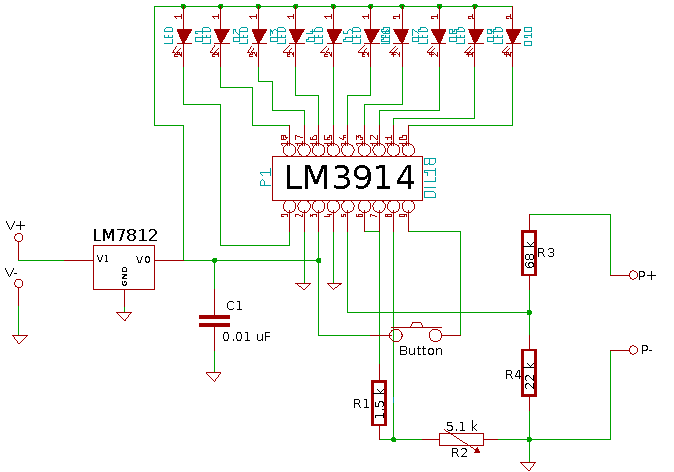
\includegraphics[scale=1.2]{images/sch.pdf}\caption{Esquemático del Circuito}
			\label{fig:circesq}
		\end{figure}

	\section{Diagrama de bloques}

		\begin{figure}[H]
			\centering
			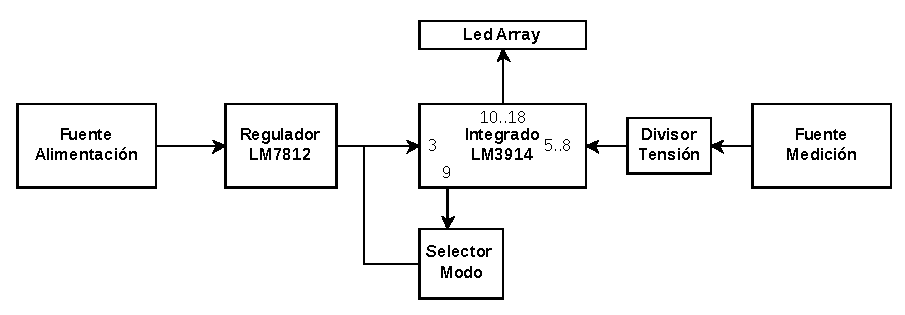
\includegraphics[scale=1.2]{images/bloque.pdf}\caption{Diagrama de Bloques}
			\label{fig:bloque}
		\end{figure}

	\begin{itemize}
		\item \textbf{Fuente de Alimentación:} La fuente que alimenta el circuito, ésta debe ser de al menos 14 V ya que el regulador de tensión es de 12V.
		\item \textbf{Regulador de Tensión:} El regulador cumple la función de mantener el equipo alimentado con 12 V, evitando daños si la entrada es mayor.
		\item \textbf{Selector Modo:} Nos permite seleccionar ambos modos de funcionamiento del circuito, tanto en "DOT" (se prende un sólo LED), como "BAR" (Se prende consecutivamente el array).
		\item \textbf{Fuente Medición:} Es la fuente de tensión a mensurar.
		\item \textbf{Divisor de Tensión:} Siendo que el integrado posee un límite de 5 V de entrada a medir, se coloca un divisor de tensión para ajustar la tensión a las especificaciones.
		\item \textbf{Array de LEDs:} Es el arreglo de LEDs luminosos en si, en este caso consiste de 10 LEDs.
		\item \textbf{Integrado LM3914: } Es el integrado encargado de la lógica del circuito.
	\end{itemize}

	\section{Desarrollo}
		Como primera instancia se debió analizar cuales serían los alcances del proyecto y ajustar las características del circuito al mismo. Lo principal a definir fue el rango de tensiones que mediriámos, decidimos utilizar el mismo rango utilizado como ejemplo en el proyecto orignal, comprendido entre los 0 y 25 V.

		Acorde al datasheet del integrado \footnote{Ver sección \ref{sec:referencias}.} el resistor $R_1$ es el encargado de regular la luminosidad de los LED. Asimismo se establece como corrientes de salida hacia los LED de un mínimo de 7 mA y un típico de 10 mA, para el proyecto establecimos un valor intermedio en $8.3$ mA. Siendo la tensión interna de referencia de $1.25$ V, por la ley de Ohm podemos calcular

		\begin{equation}
			R_1 = \frac{1.25 \: V * 10 \: LED}{8.3 \: mA} \cong 1.5 \: k \Omega
		\end{equation}

		Luego es preciso establecer un fondo de escala, la misma se calcula acorde la siguiente fórmula:

		\begin{equation}\label{eq:vref}
			V_{ref} = 1.25 \: V (1+\frac{R_2}{R_1})
		\end{equation}

		Siendo la máxima señal de entrada permitida de 5 V, para poder mensurar el rango antes mencionado (0 - 25 V) debemos emplear un divisor de tensión, para tal propósito se emplearon los resistores $R_3 = 68 \: k\Omega$ y $R_4 = 22 \: k\Omega$. Acorde a estos valores, aplicando una tensión de 25 V, sobre $R_4$ se obtendrá una caída de tensión equivalente a

		\begin{equation}
			\Delta V_{R_4} = \frac{25 \: V * 22 \: k\Omega}{90 \: k\Omega} \cong 6.1 \: V
		\end{equation}

		Si consideramos la tensión máxima de referencia, según la ecuacion \ref{eq:vref}:

		\begin{equation}
			\displaystyle R_2 = \left.  \left ( \frac{V_{ref}}{1.25 \: V}-1 \right ) * R_1 \right |_{V_{ref} = 5 \: V} = 4.5 \: k\Omega
		\end{equation}

		Siendo este resistor de un valor no comercial y con el fin de a posteriori poder realizar ajustes, empleamos un resistor variable de $10 \: k\Omega$. Teniendo todos los elementos principales ya descriptos, se prosiguió al diseño y confección del circuito.

		%Sin embargo al tener también interactuando un divisor de tensión (y resistores no exactos), empleamos un resistor variable de $10 \: k\Omega$ y aplicando una tensión de 25 V variamos la resistencia, procurando que a los 25 V se encienca el décimo LED. Una vez hecho esto, se midió la resistencia del resistor dando como resultado:

		%\begin{equation}
		%	R_2 = (3.87 \pm 0.05) \: k\Omega
		%\end{equation}

		\subsection{Construcción}

			Como primer instancia luego de adquirir todos los elementos, se armó el circuito en un \textit{protoboard} a fin de corroborar el funcionamiento de todos los componentes individual y conjuntamente.

			\begin{figure}[H]
			\centering
				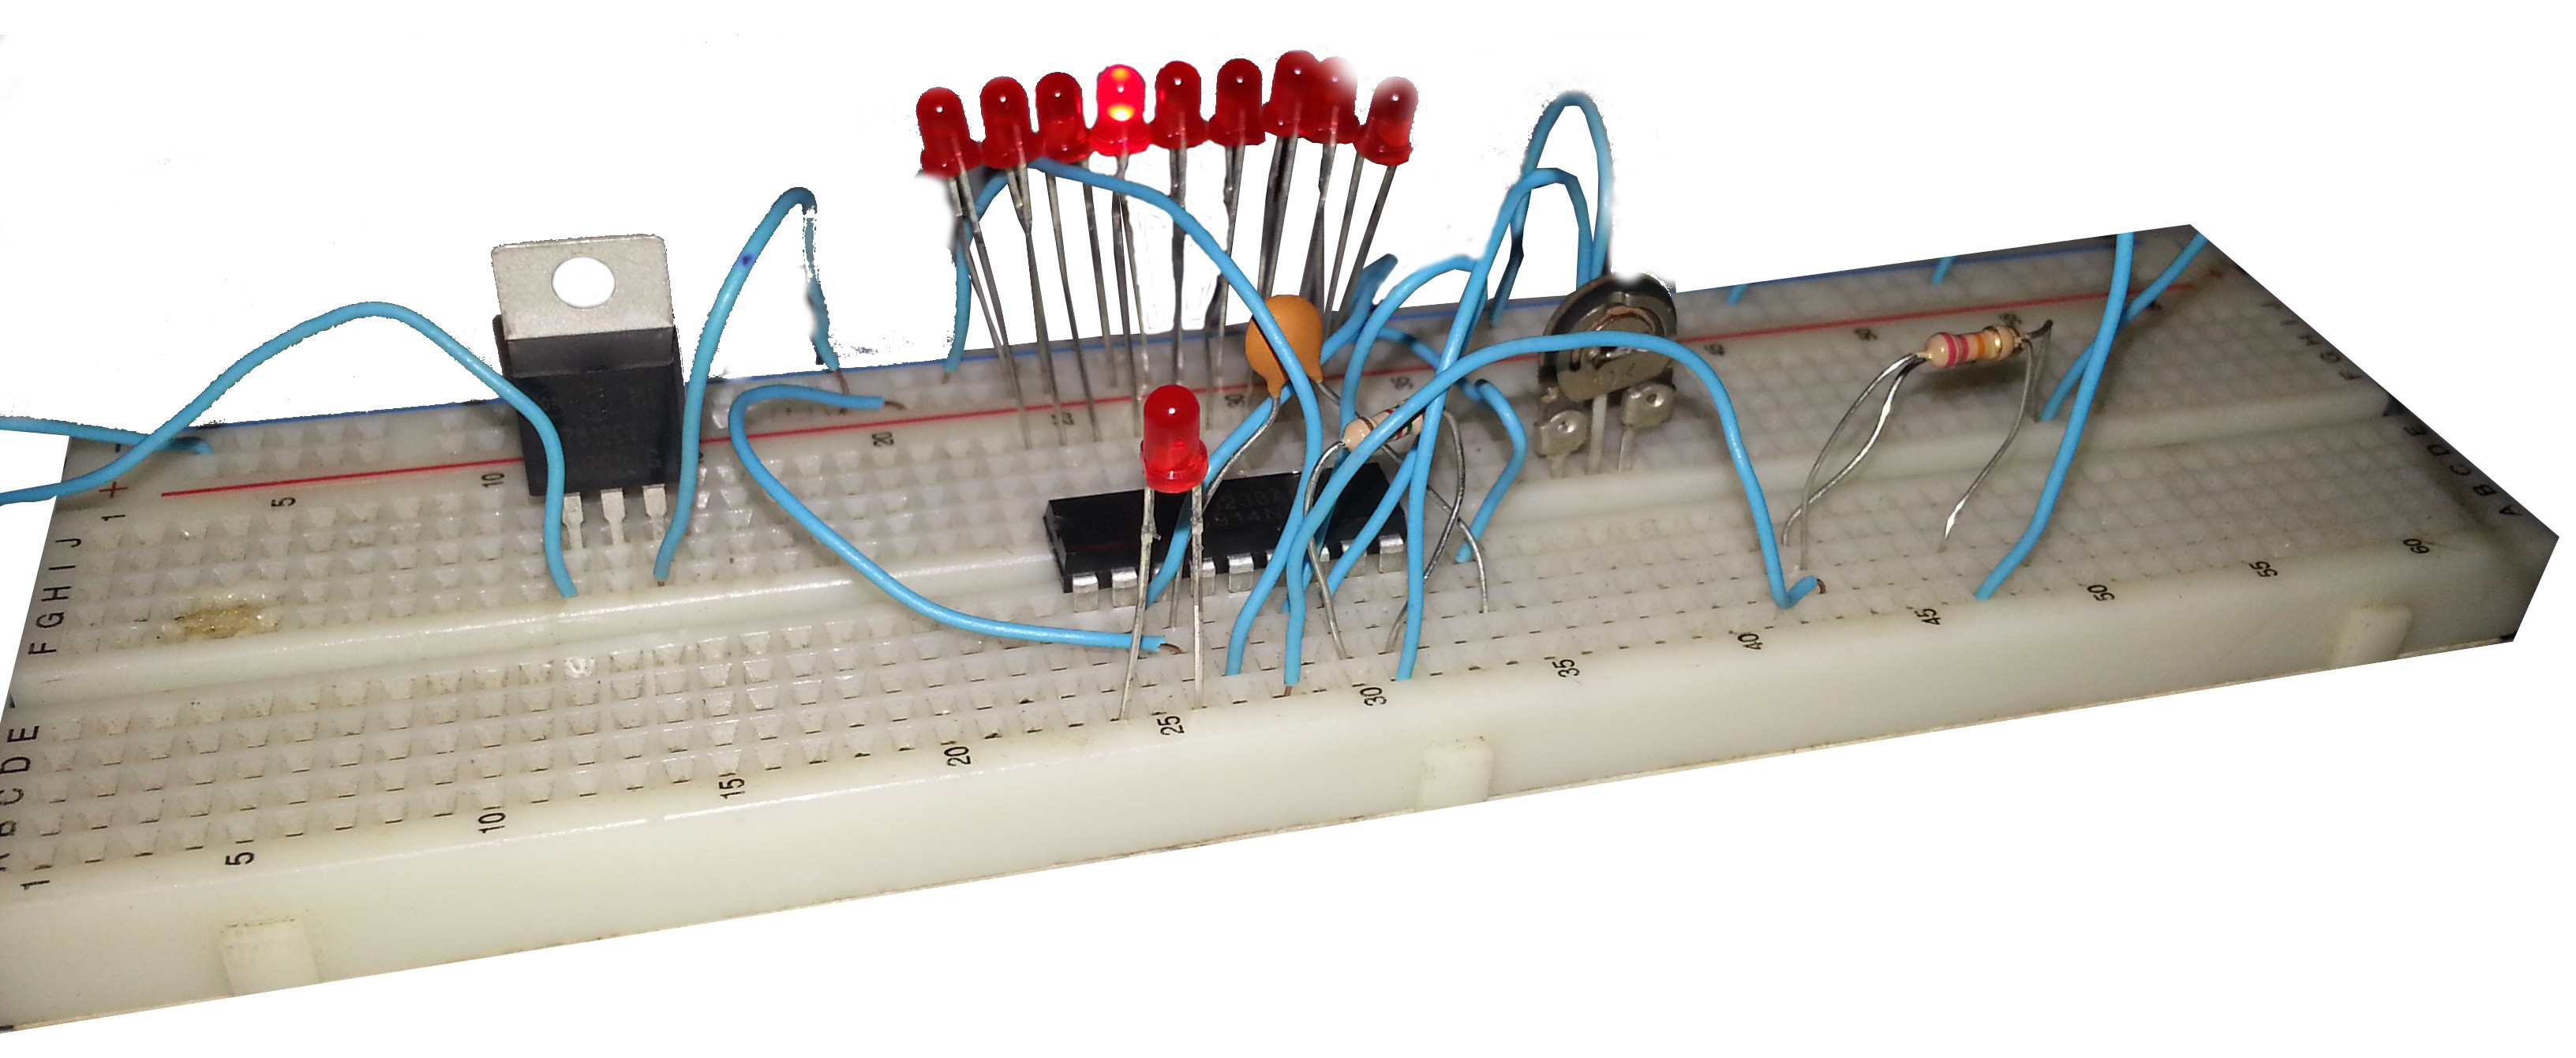
\includegraphics[scale=0.1]{images/proto_dot.jpg}\caption{Prototipo modo DOT}
			\end{figure}

			\begin{figure}[H]
			\centering
				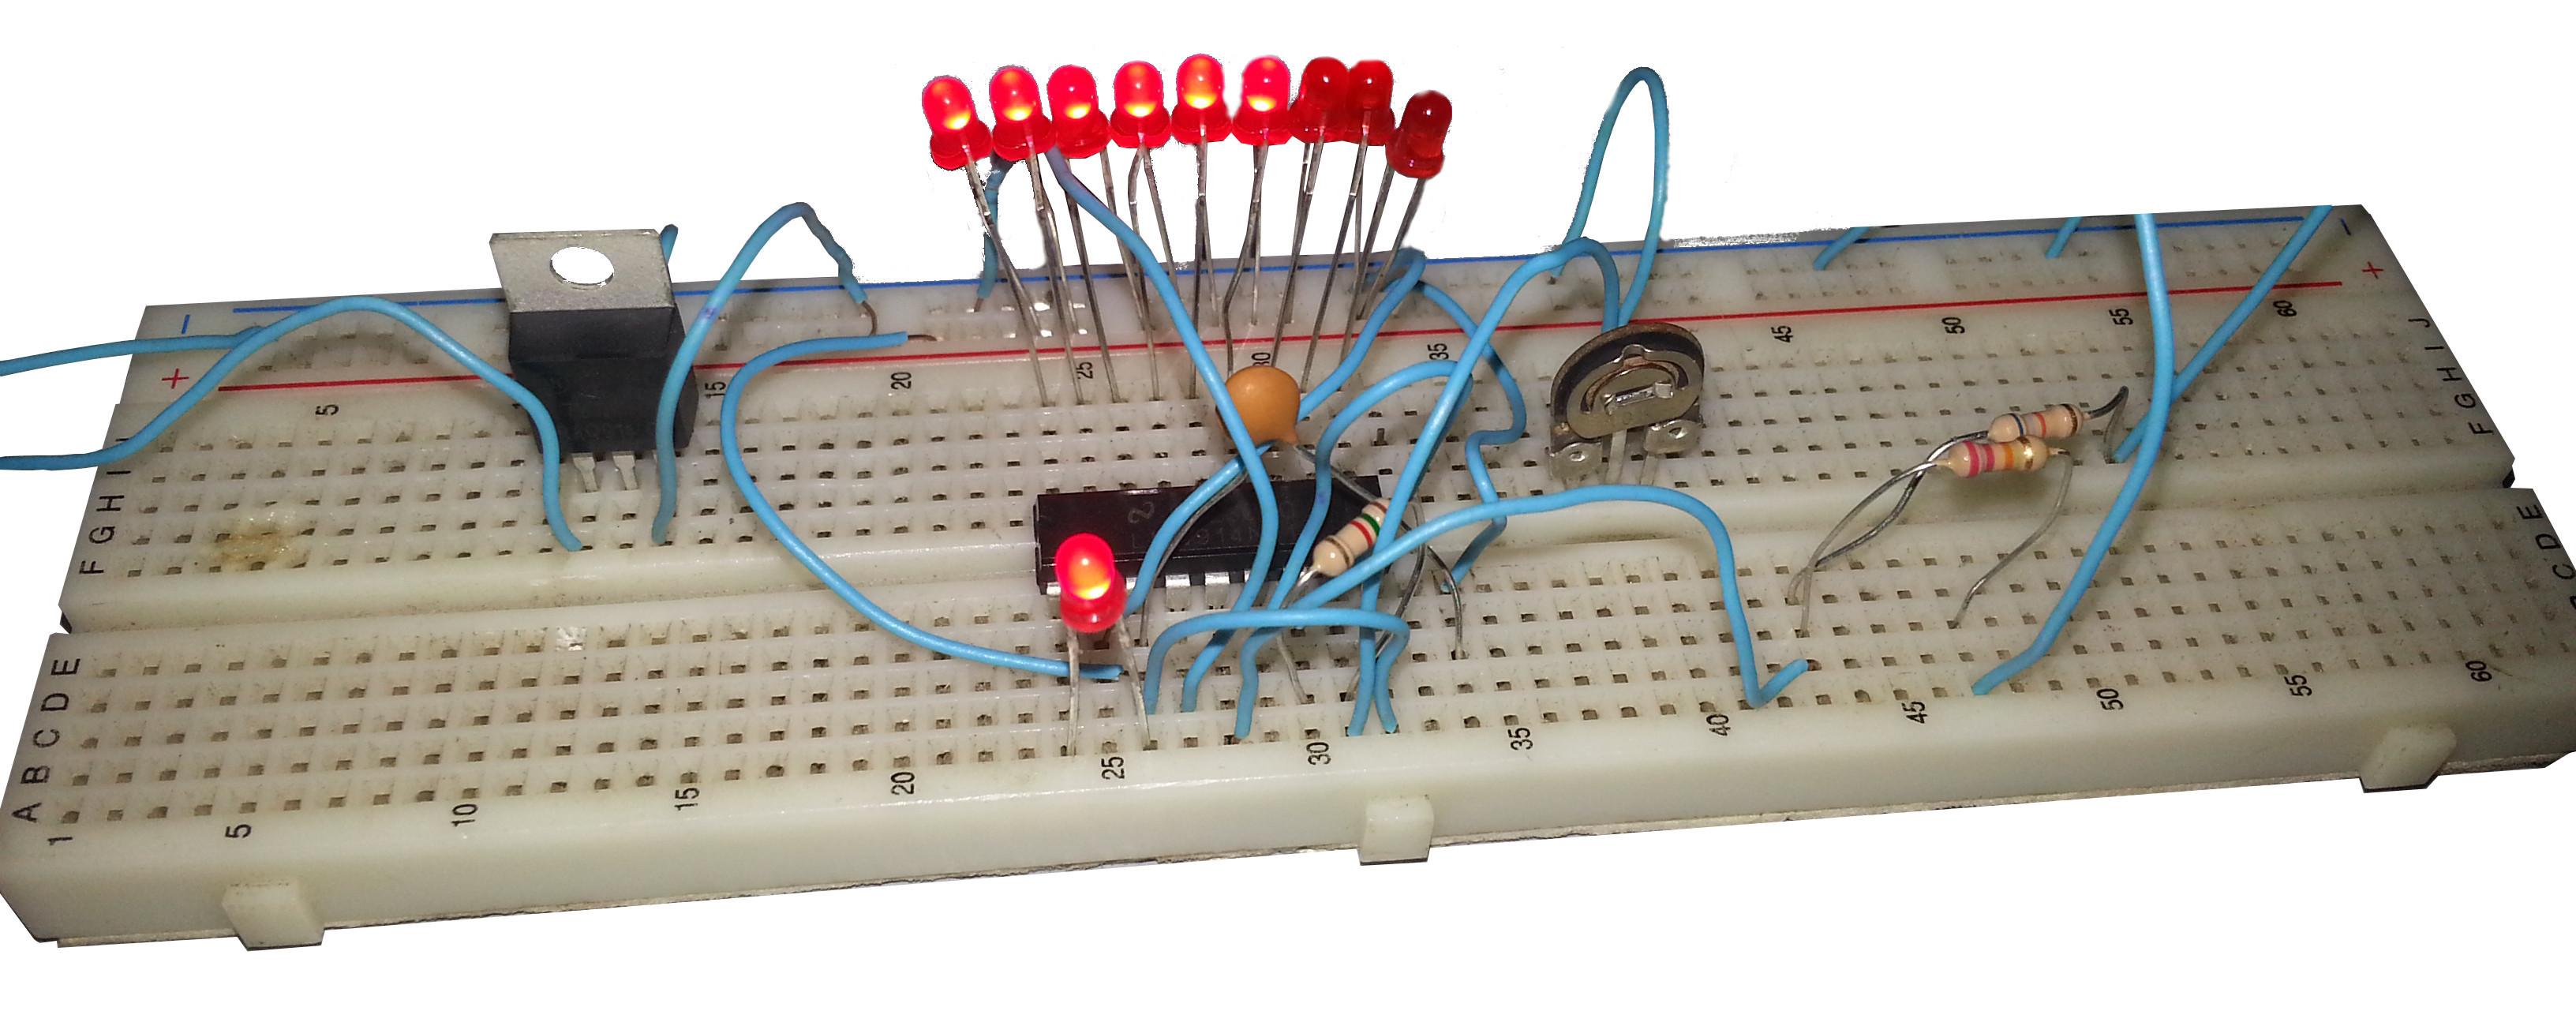
\includegraphics[scale=0.1]{images/proto_bar.jpg}\caption{Prototipo modo BAR}
			\end{figure}

			Luego aprovechando la disponibilidad de un archivo esquemático, utilizando herramientas informáticas se diseñó un circuito virtual que luego sería pasado a una plaqueta de cobre.

			\begin{figure}[H]
			\centering
				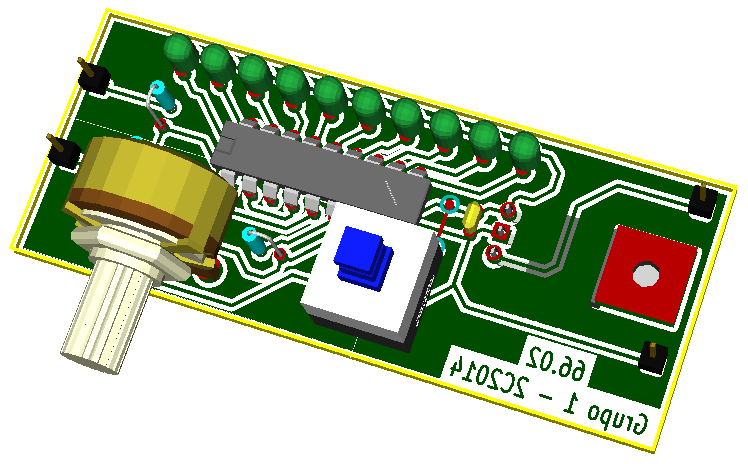
\includegraphics[scale=0.4]{images/virt_sup.png}\caption{Vista Superior Circuito Virtual}
			\end{figure}

			\begin{figure}[H]
			\centering
				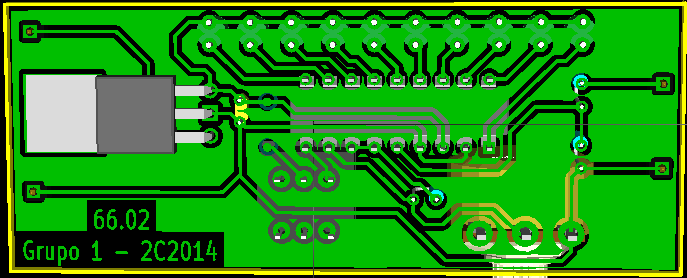
\includegraphics[scale=0.4]{images/virt_inf.png}\caption{Vista Inferior Circuito Virtual}
			\end{figure}

			Una vez conformes con el diseño, se imprimió el mismo en papel de transferencia térmico, para ser pasado a una plancha de cobre virgen y empleando ácido grabar el dibujo en la placa.

			\begin{figure}[H]
			\centering
				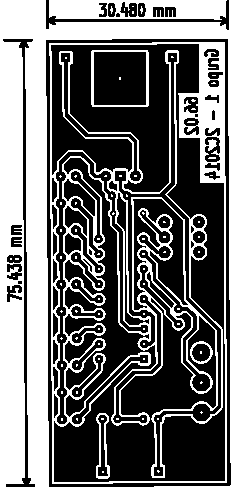
\includegraphics[scale=1,angle=-90]{images/design.pdf}\caption{Diseño Circuito}
			\end{figure}

			\begin{figure}[H]
			\centering
				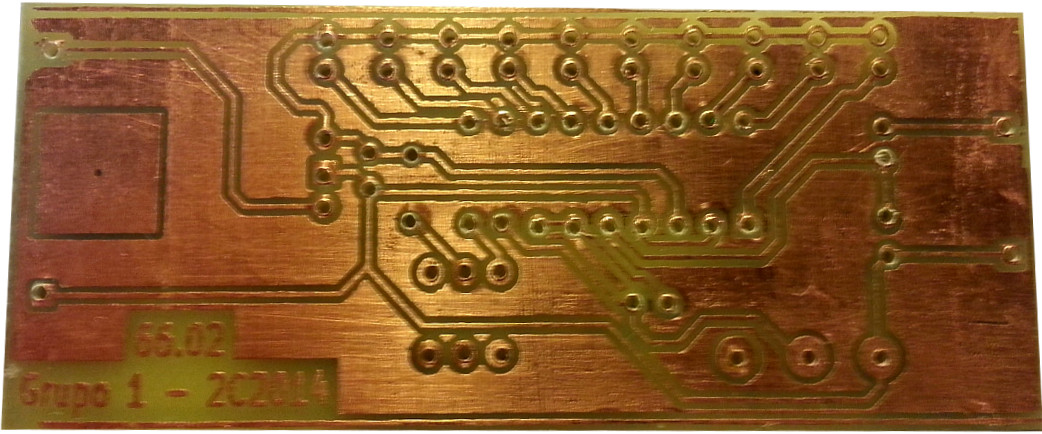
\includegraphics[scale=0.25]{images/placa_grabada.jpg}\caption{Diseño Grabado}
			\end{figure}

			\begin{figure}[H]
			\centering
				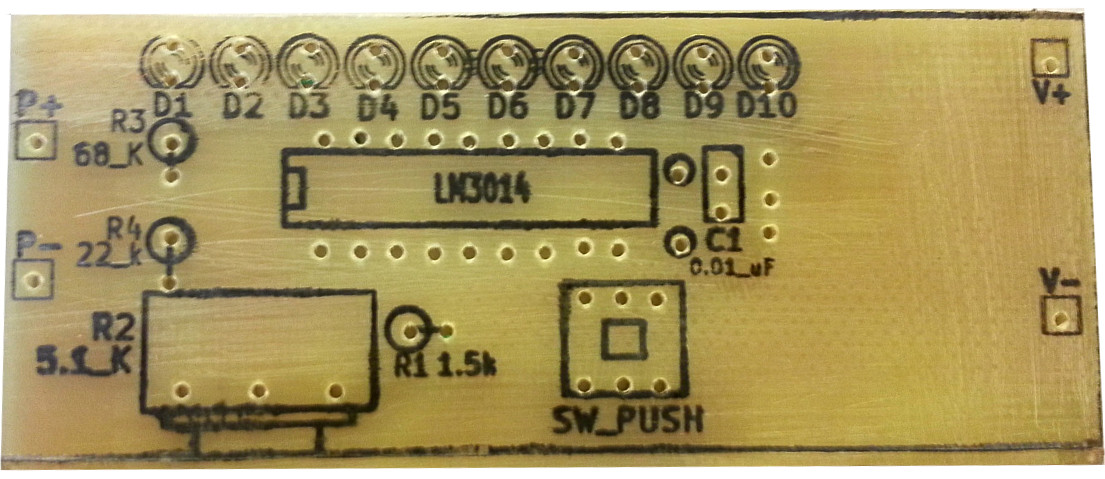
\includegraphics[scale=0.25]{images/ayuda_comps.jpg}\caption{Indicador de Componentes}
			\end{figure}

			Luego de soldar los componentes y realizar algunas reparaciones en las pistas de cobre, el circuito definitivo:

			\begin{figure}[H]
			\centering
				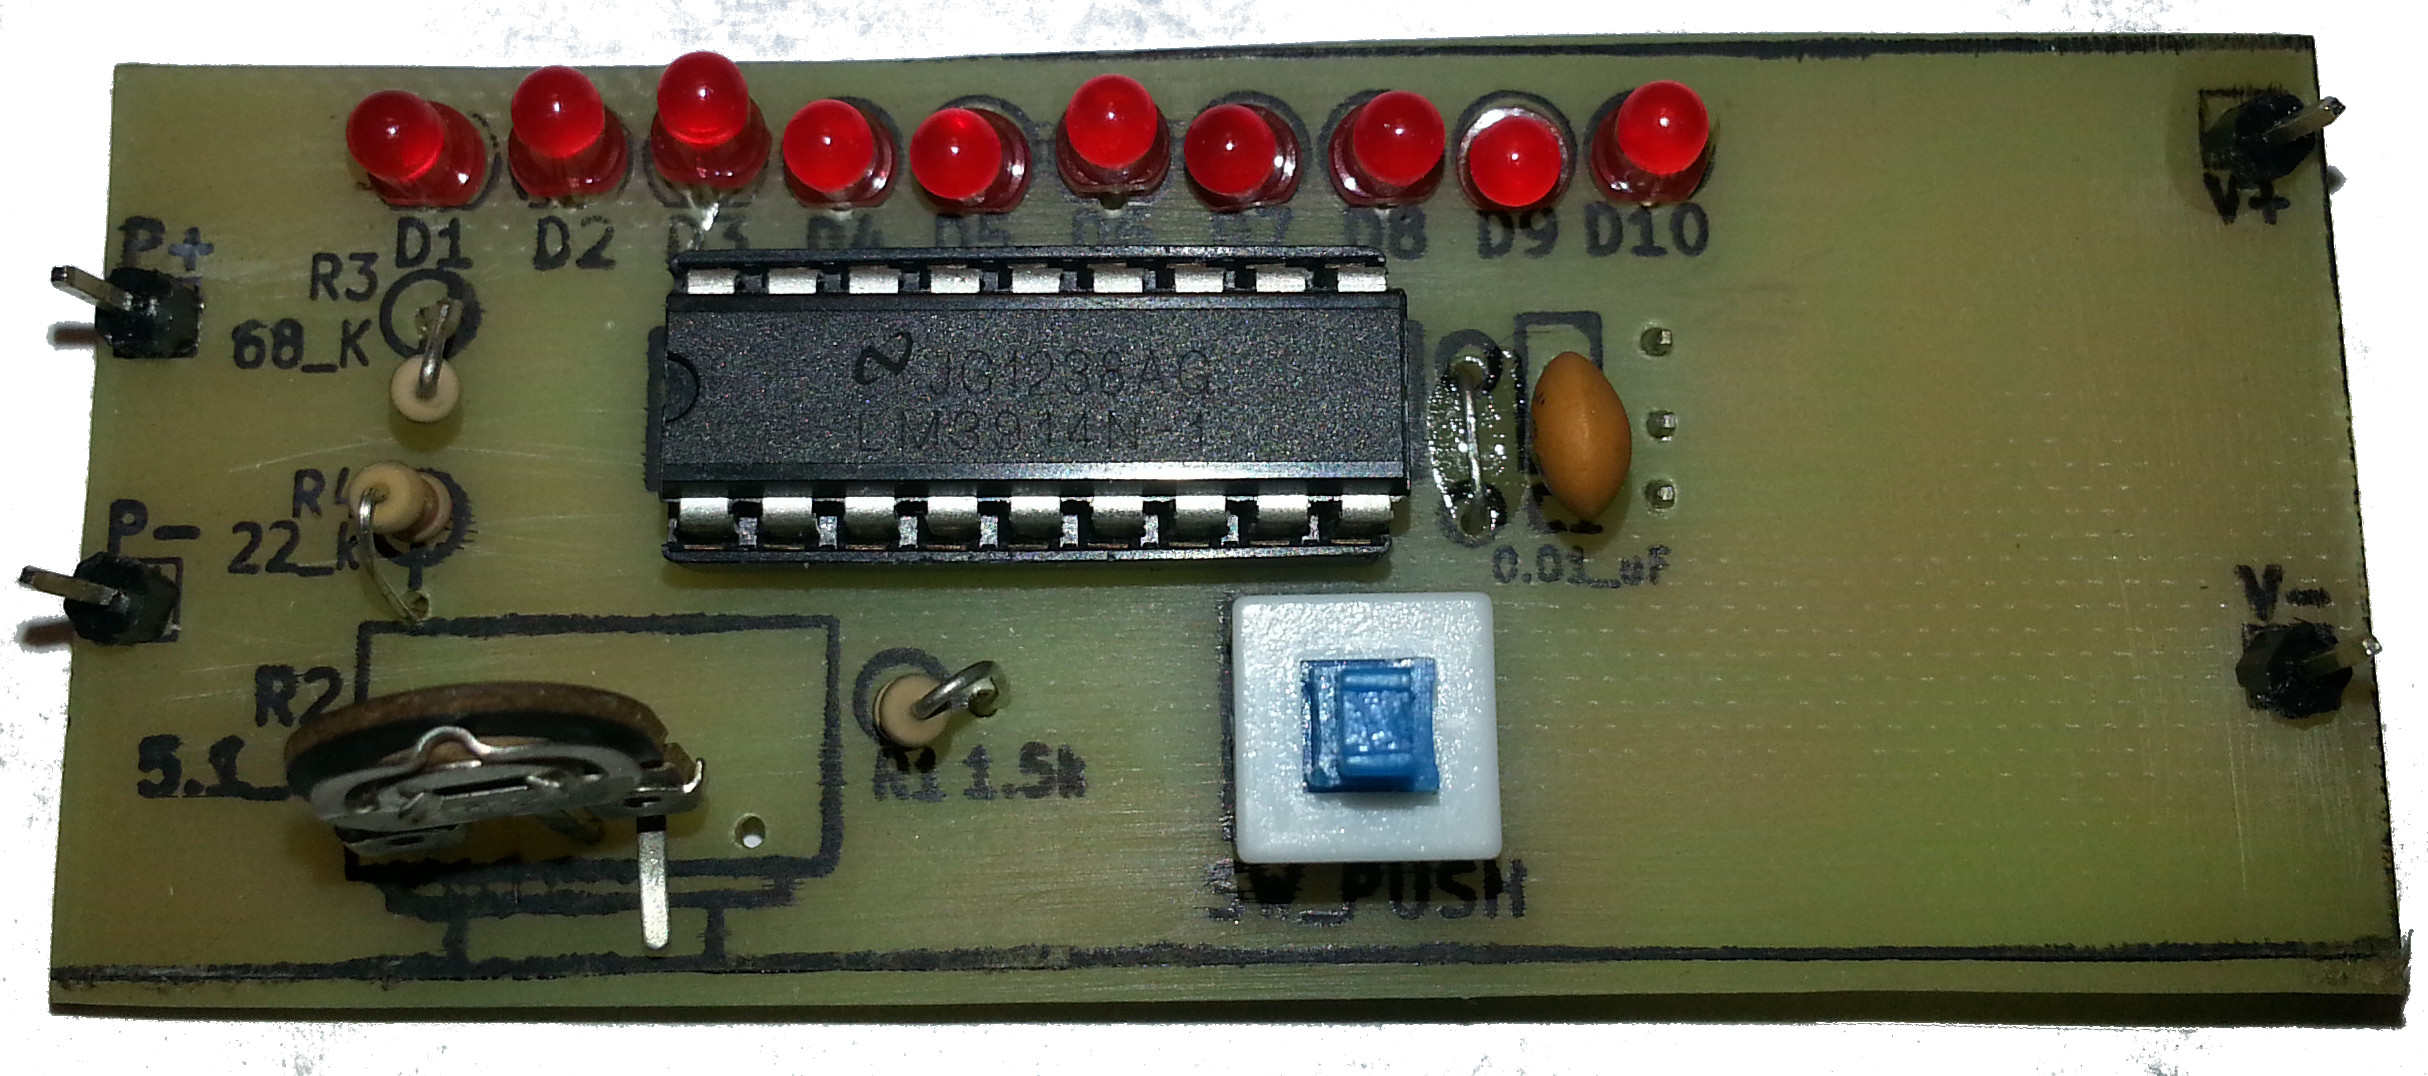
\includegraphics[scale=0.1]{images/placa_completa.jpg}\caption{Circuito Completo}
			\end{figure}

		\subsection{Materiales y Costo}

		\begin{center}
			
			{\footnotesize \begin{tabular}{ |c|l|r|r| }

			\hline
				\multicolumn{4}{|c|}{Materiales}\\ \hline
				Cantidad & Descripción & Precio Unitario [\$] & Subtotal [\$] \\ \hline
				1 & Resistor $1.5 \: k\Omega$ & & \\ \hline
				1 & Resistor variable $10 \: k\Omega$ & & \\ \hline
				1 & Resistor $68 \: k\Omega$ & & \\ \hline
				1 & Resistor $22 \: k\Omega$ & & \\ \hline
				10 & LED Rojo 3 mm & & \\ \hline
				1 & Capacitor Cerámico $0.01 \: \mu F$ & & \\ \hline
				1 & Pulsador 6 pines & & \\ \hline
				1 & Integrado LM3914 & & \\ \hline
				1 & Regulador LM7812 & & \\ \hline
				1 & Base Integrado 18 pines & & \\ \hline
				1 & Placa Cobre 10x10 cm & & \\ \hline
				1 & Hoja Transferencia Térmica & 10 & 10\\ \hline


			\end{tabular}}\captionof{table}{Lista de Precios}\label{tab:costo}
			\end{center}

	\newpage
	\section{Escalabilidad}
		\label{sec:escalabilidad}

	\newpage
	\section{Referencias}
		\label{sec:referencias}

\end{document}
